\documentclass{article}
\usepackage{graphicx, amsmath}
\graphicspath{ {./images/} }

\title{Elasticity of Supply and Demand Problem Set Solutions}
\author{Principles of Microeconomics}
\date{\today}

\begin{document}

\maketitle

\begin{enumerate}

\item (b)

	\begin{gather*}
	\% \Delta P = \frac{24 - 16}{\frac{24 + 16}{2}} = \frac{8}{20} = \frac{2}{5} \\
	\% \Delta Q = \frac{110 - 90}{\frac{110 + 90}{2}} =  \frac{20}{100} = \frac{1}{5} \\
	\text{Price Elasticity of Supply} = \frac{\% \Delta Q}{\% \Delta P} = \frac{1}{2} = 0.5.
	\end{gather*}
	
\item (c) -- If the price elasticity of supply is zero, that means the supply curve is perfectly inelastic, and perfectly inelastic supply is vertical.

\item (c) -- The ability of firms to enter and exit a market in the long run gives sellers more flexibility to change the amount they produce, so it makes the supply curve more elastic.

\newpage

%\item Meredith:
%
%\begin{figure}[ht]
%\centering
%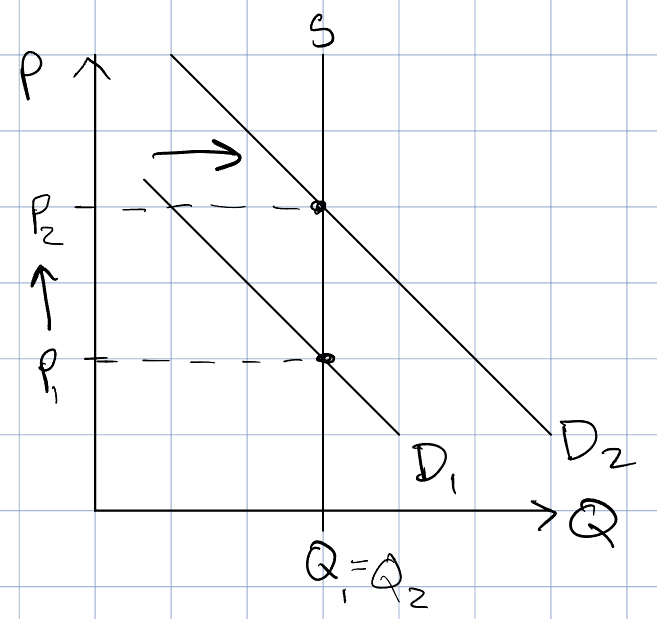
\includegraphics[width = 0.3\textwidth]{problem4_meredith}
%\end{figure}
%
%Miranda:
%
%\begin{figure}[ht]
%\centering
%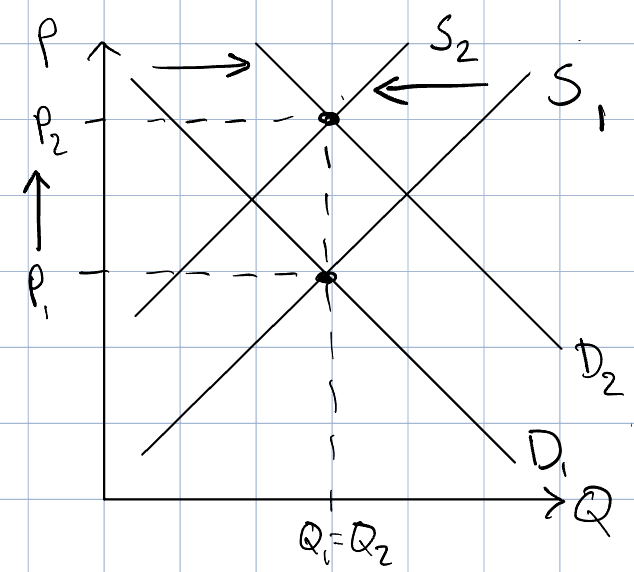
\includegraphics[width = 0.3\textwidth]{problem4_miranda}
%\end{figure}
%
%Owen:
%
%\begin{figure}[ht]
%\centering
%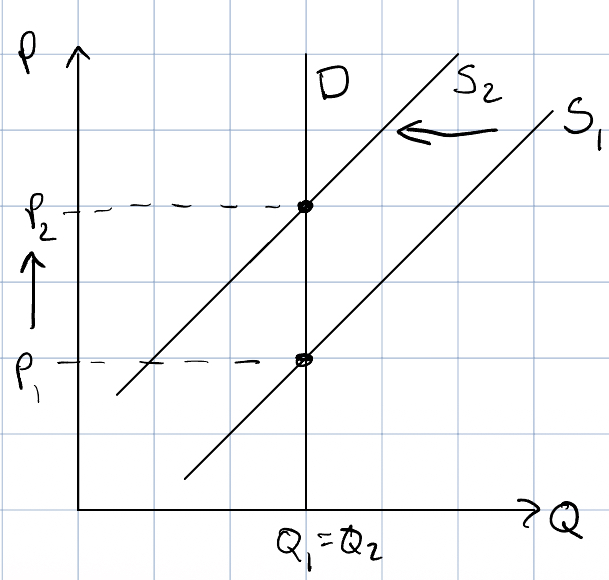
\includegraphics[width = 0.3\textwidth]{problem4_owen}
%\end{figure}

\item \phantom{x} \\

\begin{center}
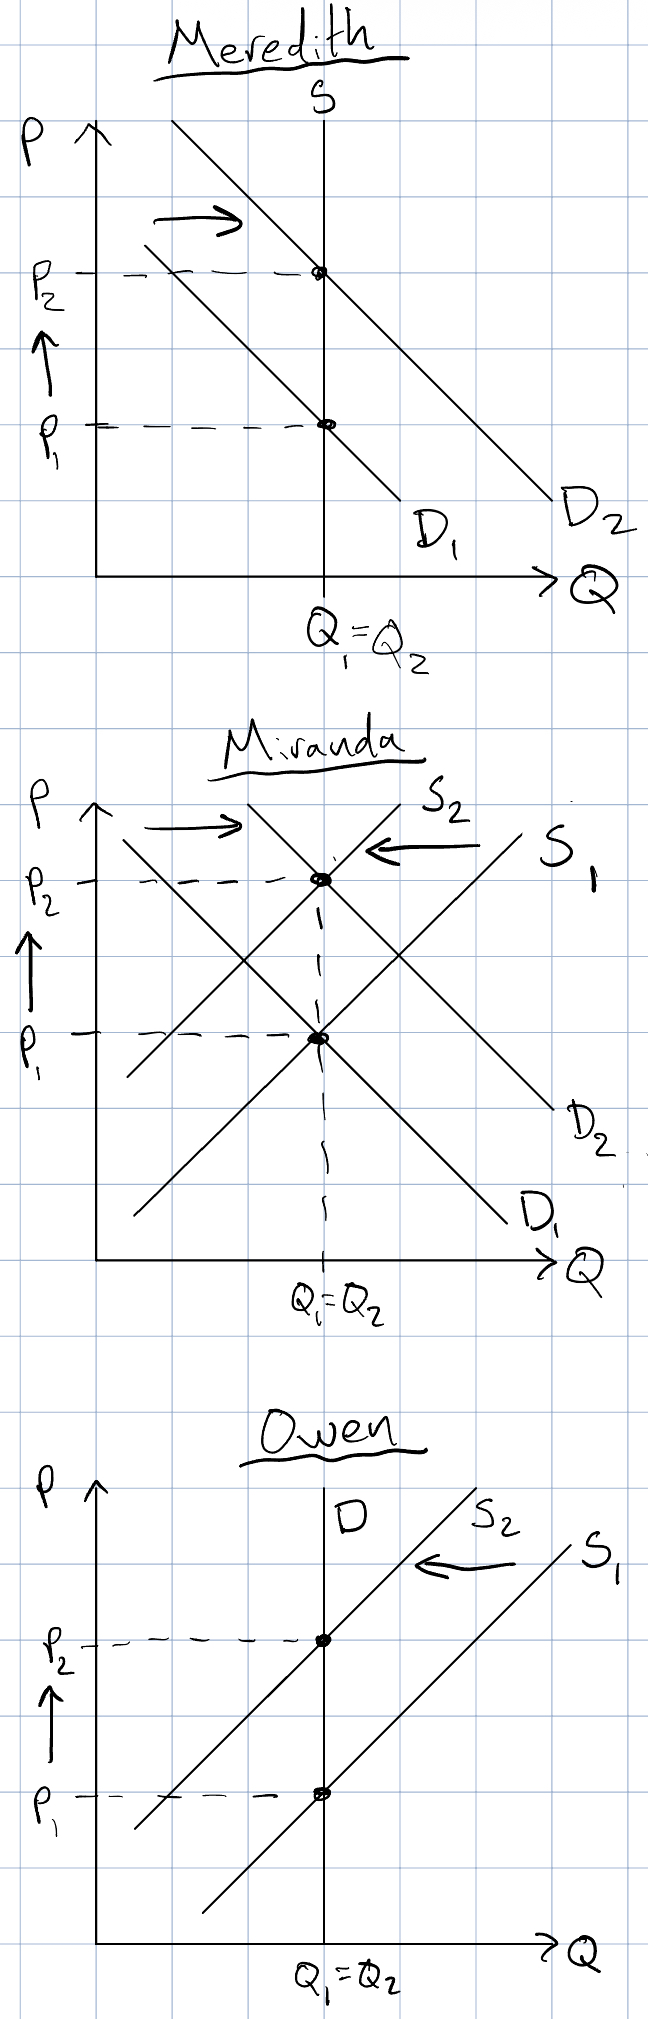
\includegraphics[width = 0.45\textwidth]{problem4}
\end{center}

\item

	\begin{enumerate}
	
	\item 
	
		\begin{gather*}
		\% \Delta Q = -0.043 \\
		\% \Delta P = \frac{1.5 - 1.25}{\frac{1.5 + 1.25}{2}} = \frac{0.25}{1.375} \approx 0.18 \\
		\eta = \left| \frac{\% \Delta Q}{\% \Delta P} \right| \approx 0.24
		\end{gather*}
		
	\item Based on my estimate, demand for subway rides is inelastic, so when the Transit Authority raises fares, we should expect revenue to increase. That's because quantity demanded will decrease proportionately less than fares will increase. 
	
	\item The estimate might be unreliable because there could be other reasons for the decrease in ridership in December. For example, it's possible that so many people take vacation in December that subway ridership drops significantly. (This question doesn't test anything we've learned. It's just a common sense question that hints at econometrics, a statistics course you'll take in college if you choose to major in economics.) 
	
	\end{enumerate}
	
\item It depends on the price elasticity of demand for museum admission. If demand is elastic, the museum should decrease the price of admission because the quantity of admits will increase proportionately more than the drop in price. If demand is inelastic, the museum should increase the price of admission because the quantity of admits will decrease proportionately less than the increase in price. I imagine demand for museum admission is elastic because it's a highly substitutable activity.

\end{enumerate}

\end{document}